\section{Cross-Asset Correlations}
The correlation matrix below is computed on daily changes across the entire sample (April 2018 -- April 2023).

\subsection*{Strong Positive Correlations (daily changes)}
\begin{itemize}
  \item ITRX IG vs ITRX XO: \(+0.9247\)
  \item CDX IG vs CDX HY: \(+0.8240\)
  \item DEM10 vs DEM2: \(+0.8192\)
  \item UST10 vs UST2: \(+0.7525\)
\end{itemize}
Interpretation: these are mostly same-asset-family and same-region risk-factor structures (credit with credit, curve points with curve points).

\subsection*{Strong Negative Correlations (daily changes)}
\begin{itemize}
  \item S\&P vs CDX HY: \(-0.7810\)
  \item S\&P vs VIX: \(-0.7746\)
  \item ESTX600 vs ITRX XO: \(-0.7505\)
  \item S\&P vs CDX IG: \(-0.7104\)
\end{itemize}
Interpretation: classical risk-on/risk-off behavior where equity up-days typically coincide with tighter credit spreads and lower implied volatility.

\begin{figure}[H]
  \centering
  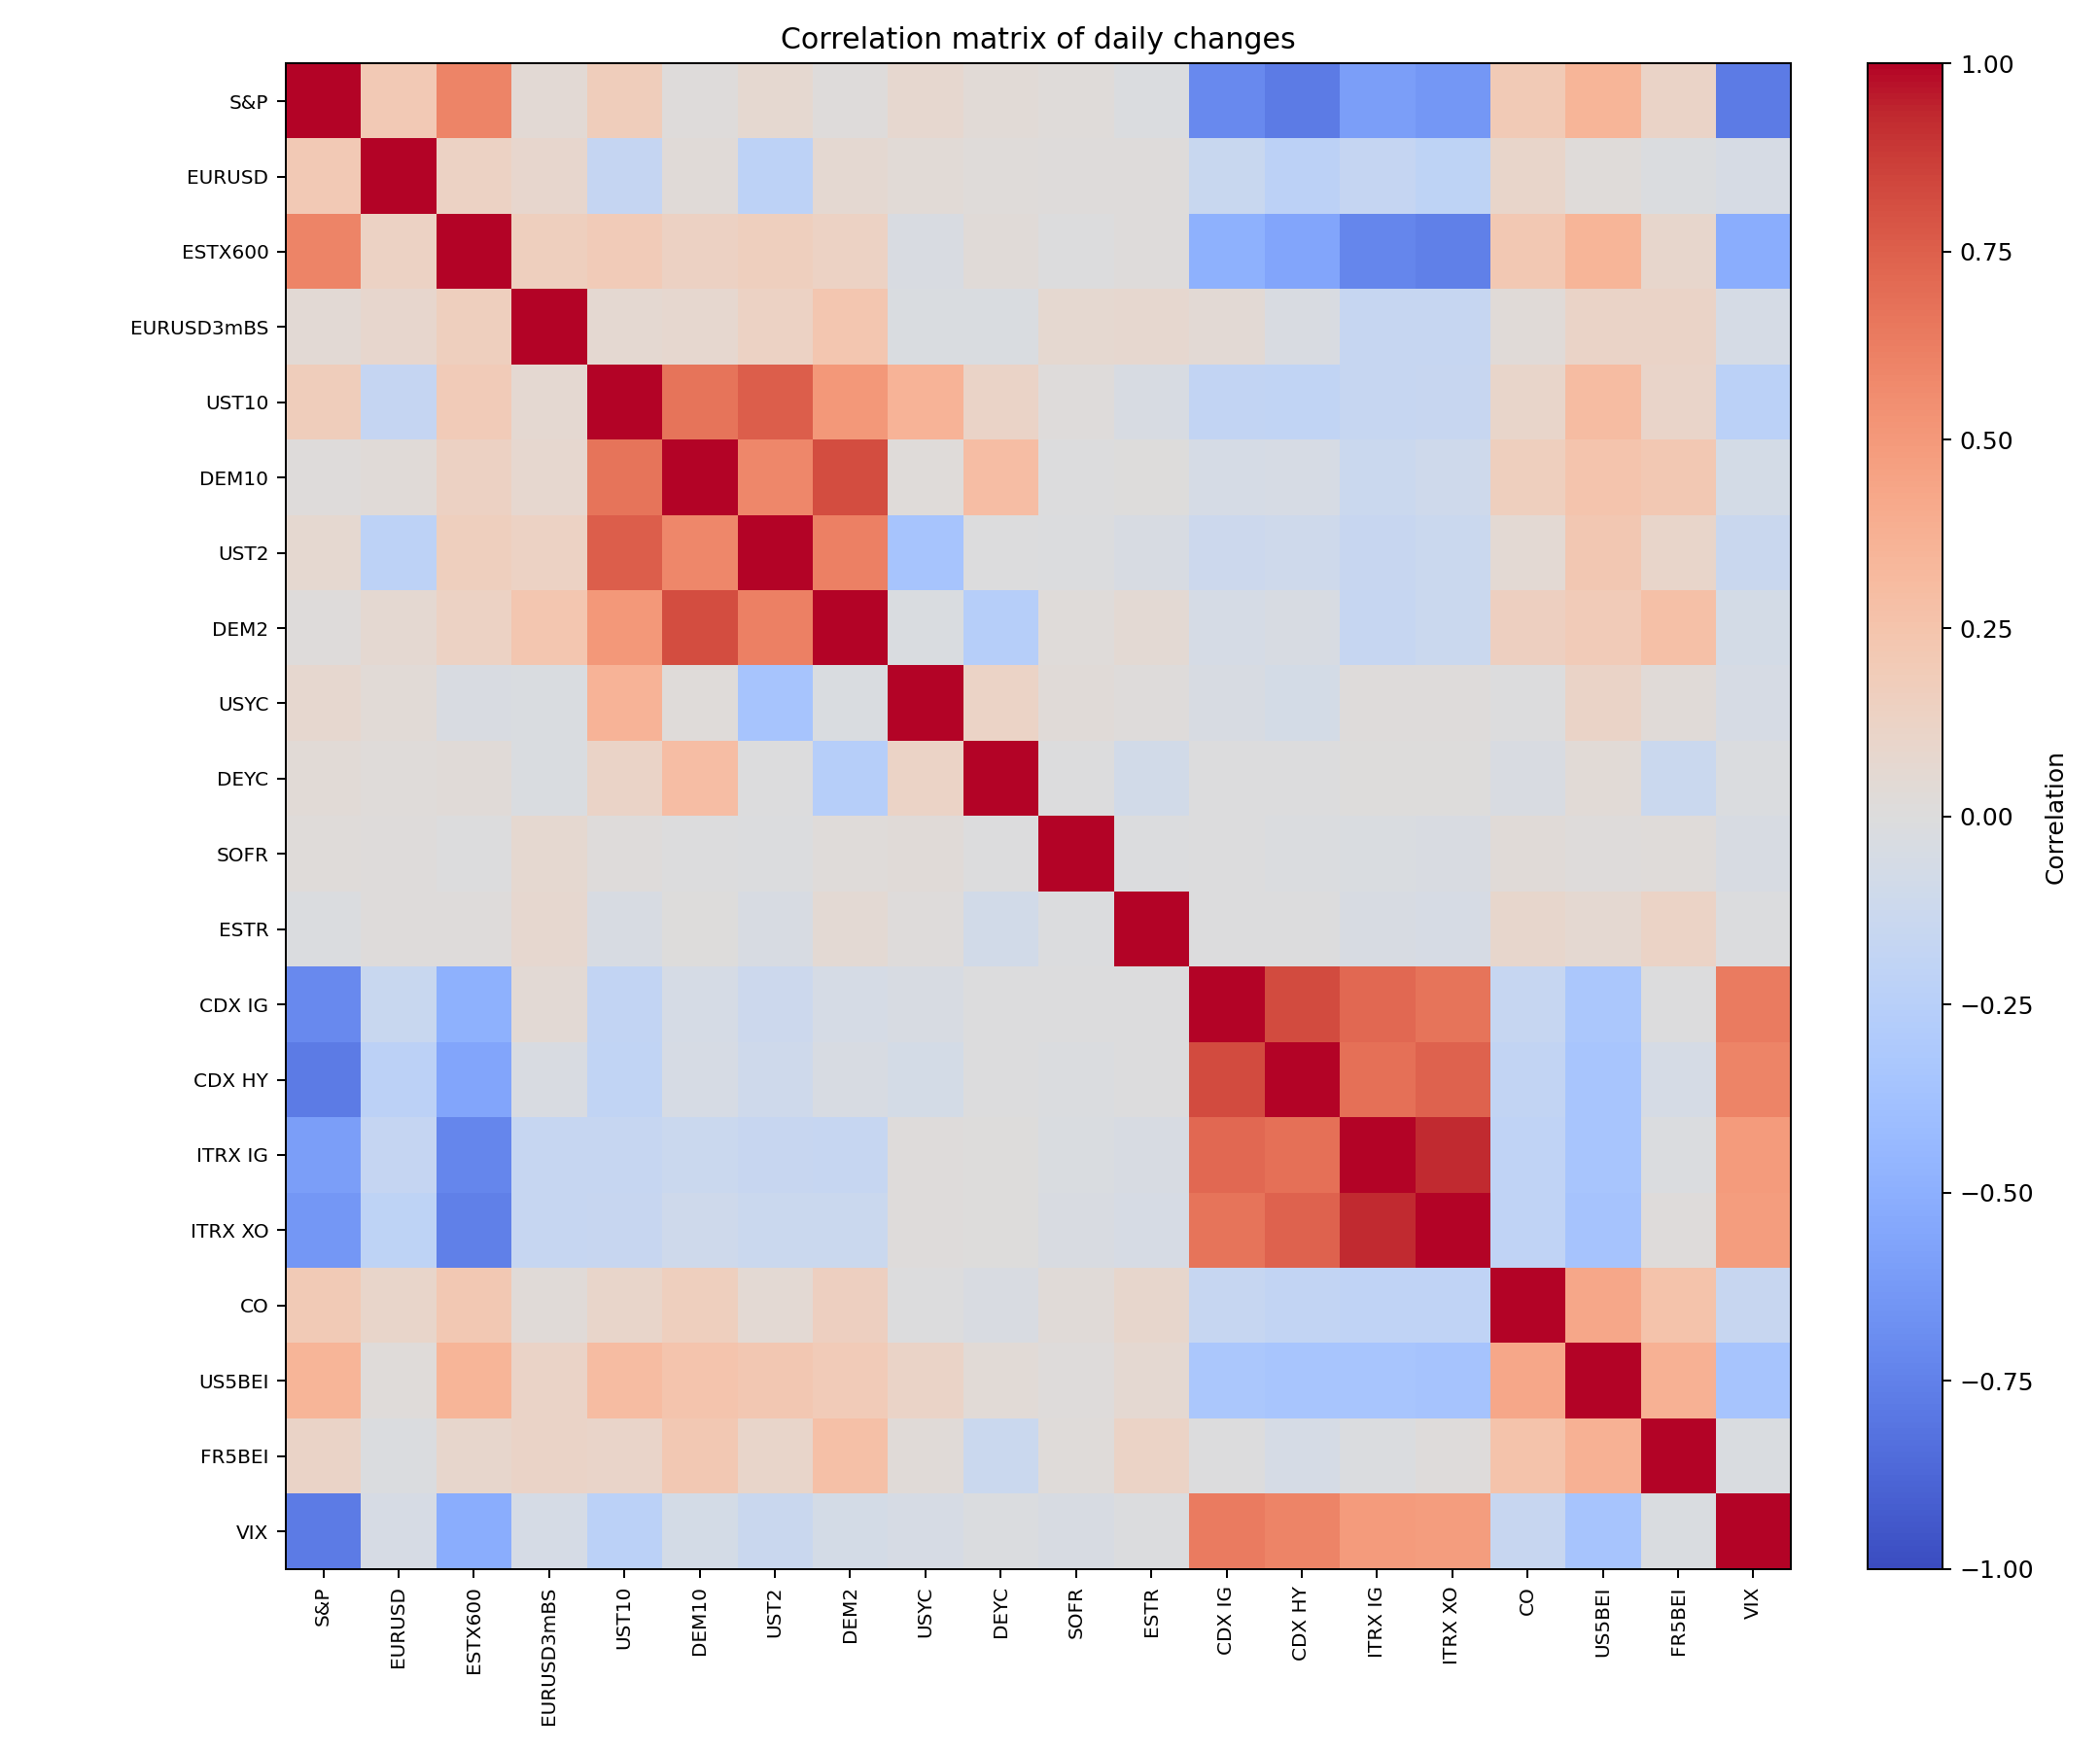
\includegraphics[width=\textwidth]{../../../output/figures/corr_heatmap_changes.png}
  \caption{Correlation matrix of daily changes across all variables.}
\end{figure}
